\documentclass[11pt]{article}
\usepackage{natbib}
\usepackage{url}
\usepackage[utf8]{inputenc} % Codificación
\usepackage{amsmath}
\usepackage{graphicx}
\graphicspath{{images/}} % Carpeta en la cual se van a buscar las imagenes
\usepackage{subfigure}	% Permite la Inclusión de subfiguras
%\usepackage{parskip} % Borrar identación de parrafos.
\setlength{\parskip}{3mm} % Longitud del espaciado entre parrafos
\usepackage[hidelinks]{hyperref} % Referencias (links)
\usepackage{fancyhdr}
\usepackage{vmargin}
\setpapersize{A4} % Formato del papel - A4
\setmarginsrb{3 cm}{2.5 cm}{3 cm}{2.5 cm}{1 cm}{1.5 cm}{1 cm}{1.5 cm} % Margenes
\usepackage{paralist} % Permite un mayor control sobre las listas
\usepackage{textcomp,marvosym,pifont} % Generación de símbolos especiales
\usepackage[usenames,dvipsnames,svgnames,x11names,table]{xcolor}

%%%%%%%%%%%%%%%%%%%%%%%%%%%%%%%%%%%%%%%%%%%%%%%%%%%%%%%%%%%%%%%%%%%%%%%%%%%%%%%%%%%%%%%%%
% Complemento para insertar código en la memoria:
% A partir de 'Listados de código cómodos y resultones con listings' de David Villa
% http://crysol.org/es/node/909

\usepackage{color}
\definecolor{gray97}{gray}{.97}
\definecolor{gray75}{gray}{.75}
\definecolor{gray45}{gray}{.45}

\usepackage{listings}
\lstset{ frame=Ltb,
	framerule=0pt,
	aboveskip=0.5cm,
	framextopmargin=3pt,
	framexbottommargin=3pt,
	framexleftmargin=0.4cm,
	framesep=0pt,
	rulesep=.4pt,
	backgroundcolor=\color{gray97},
	rulesepcolor=\color{black},
	texcl=true,
	%
	stringstyle=\ttfamily,
	showstringspaces = false,
	basicstyle=\small\ttfamily,
	commentstyle=\color{gray45},
	keywordstyle=\bfseries,
	%
	numbers=left,
	numbersep=15pt,
	numberstyle=\tiny,
	numberfirstline = false,
	breaklines=true,
}

% minimizar fragmentado de listados
\lstnewenvironment{listing}[1][]
{\lstset{#1}\pagebreak[0]}{\pagebreak[0]}

\lstdefinestyle{consola}
{basicstyle=\scriptsize\bf\ttfamily,
	backgroundcolor=\color{gray75},
}

\lstdefinestyle{C}
{language=C,
}
%%%%%%%%%%%%%%%%%%%%%%%%%%%%%%%%%%%%%%%%%%%%%%%%%%%%%%%%%%%%%%%%%%%%%%%%%%%%%%%%%%%%%%%%%

\usepackage{float} % Permite usar H en las figuras, de manera que se coloquen en la posición exacta en la que están en el código.


% Añade un comando para crear indicaciones de pulsación de teclas
\usepackage{tikz} % Paquete especializado en gráficos
\usetikzlibrary{shadows} % Necesario para poder crear nuevo comando de indicación de pulsación de tecla.
\newcommand*\tecla[1]{%   
	\tikz[baseline=(key.base)]
	\node[%
	draw,
	fill=white,
	drop shadow={shadow xshift=0.25ex,shadow yshift=-0.25ex,fill=black,opacity=0.75},
	rectangle,
	rounded corners=2pt,
	inner sep=1pt,
	line width=0.5pt,
	font=\scriptsize\sffamily
	](key) {#1\strut}
	;
}

\newif\ifspanish % Condicional que permite seleccionar el lenguage.
\spanishtrue


%%%%%%%%%%%%%%%%%%%%%%%%%%%%%%%%%%%%%%%%%%%%%%%%%%%%%%%%%%%%%%%%%%%%%%%%%%%%%%%%%%%%%%%%%
%%%%%%%%%					Principales variables del documento					%%%%%%%%%

\title{Práctica 4. Gestión de prioridad de tráfico en IP.}							% Titulo
\author{Alberto Salas Seguín y Marcos López Sobrino.}							% Autor
\date{\today}											% Fecha
\newcommand{\subject}{Planificación e Integración de Sistemas y Servicios.}						% Asignatura
\newcommand{\course}{4º Grado en Ingeniería Informática.}		% Curso

%\spanishfalse	% Descomentar esta línea si el trabajo está en inglés

%%%%%%%%%%%%%%%%%%%%%%%%%%%%%%%%%%%%%%%%%%%%%%%%%%%%%%%%%%%%%%%%%%%%%%%%%%%%%%%%%%%%%%%%%

\ifspanish
	\usepackage[spanish]{babel} % Paquete de español
	\newcommand{\dateText}{Fecha:}
	\renewcommand{\lstlistingname}{Listado} % Renombrar listados para que aparezcan en español.
	% Algoritmos
	\usepackage[ruled,vlined,spanish]{algorithm2e} % Permite pseudocódigos. NECESARIO INSTALAR texlive-science (sudo apt-get install texlive-science)
\else
	\usepackage[english]{babel} % Paquete de inglés
	\newcommand{\dateText}{Date:}
	% Algoritmos
	\usepackage[ruled,vlined,english]{algorithm2e}
\fi

\makeatletter
\let\thetitle\@title
\let\theauthor\@author
\let\thedate\@date
\makeatother

\pagestyle{fancy}
\fancyhf{}
\rhead{\theauthor}
\lhead{\thetitle}
\cfoot{\thepage}

\begin{document}
\begin{titlepage}
	\centering
    
\includegraphics[scale = 0.25]{esilogo.png}\\[1.0 cm]	% Logo de la universidad
    \textsc{\LARGE Universidad de Castilla-La Mancha}\\[0.5 cm]	% Nombre de la universidad
    \textsc{\LARGE Escuela Superior de Informática}\\[2.0 cm]
	\textsc{\Large \textbf{\subject}}\\[0.5 cm]				% Asignatura
	\textsc{\large \course}\\[0.5 cm]						% Curso
	\rule{\linewidth}{0.2 mm} \\[0.4 cm]
	{ \huge \bfseries \thetitle}\\
	\rule{\linewidth}{0.2 mm} \\[1.5 cm]
	
	\begin{minipage}{0.4\textwidth}
		\begin{flushleft} \large
			\emph{Autor:}\\
			\textbf{\theauthor}
			\end{flushleft}
			\end{minipage}~
			\begin{minipage}{0.4\textwidth}
			\begin{flushright} \large
			\emph{\dateText} \\
			\thedate
		\end{flushright}
	\end{minipage}\\[1.5 cm]
 
	\vfill
	
\end{titlepage}

\section{Entorno de trabajo.}
El entorno de trabajo utilizado han sido 3 máquinas virtuales gestionadas mediante Vagrant, con la imagen \textbf{\textit{ubuntu/trusty64}}. Una de ellas actúa como cliente, otra como servidor y otra como router entre ambas. A continuación, explicamos la configuración de las redes, de las máquinas, y los paquetes instalados.
\begin{figure}[hbtp]
\centering
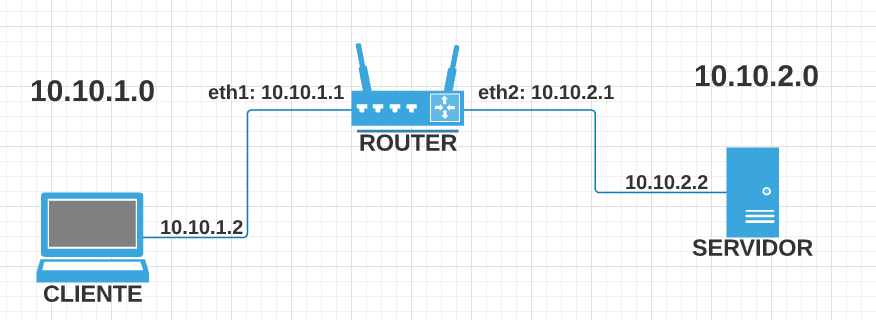
\includegraphics[scale=0.5]{top.png}
\caption{Topología de la red.}
\end{figure}

\subsection{Cliente y servidor.} 
Como vemos en la figura anterior, la red del cliente, que corresponde a la interfaz \textbf{eth1} del router, tiene como IP \textbf{10.10.1.0}; mientras que la red del servidor, que corresponde a la interfaz \textbf{eth2} del router, tiene como IP \textbf{10.10.2.0}. \\ \\
Para el correcto funcionamiento de las comunicaciones, hay que indicarle a la máquina cuál es la ruta por defecto, para ello, se ejecutan los siguientes comandos:

\begin{lstlisting}[style=C, numbers=none]
$ sudo ip route del default dev eth0
$ sudo ip route add default via <ip_router> dev eth1
\end{lstlisting}
donde \textit{ip\_router} sería la dirección IP de la interfaz del router dentro de la red correspondiente. \\ \\
\newpage
Los paquetes necesarios para el funcionamiento de la práctica en el caso del cliente y el servidor son:
\begin{itemize}
\item \textbf{iptables}
\item \textbf{iperf}
\item \textbf{sip-tester}
\end{itemize}

\subsection{Router.}
A la máquina del router se le ha instalado un entorno gráfico para poder usar cómodamente la herramienta \textbf{Wireshark}. Además, se le han asignado 2048 MB de RAM. Por otra parte, se ha configurado las interfaces de red con la dirección \textbf{.1} de la red correspondiente, tal y como vemos en la figura. Adicionalmente, para que la máquina actúe como router se debe activar el \textbf{IP forwarding}, para ello, en el playbook correspondiente del router se ha añadido una regla específica. \\ \\
Por último, en el router se han instalado los siguientes paquetes:
\begin{itemize}
\item Para la interfaz gráfica:
	\begin{itemize}
		\item \textbf{xorg}
		\item \textbf{gnome-core}
		\item \textbf{gnome-system-tools}
		\item \textbf{gnome-app-install}
	\end{itemize}
\item \textbf{wireshark}
\item \textbf{iptables}			
\end{itemize}

\subsection{Archivos de configuración e inicialización.}
Todo lo anterior se recoge en el archivo \textbf{\textit{Vagrantfile}} y los distintos \textbf{\textit{playbooks}}, que se pueden encontrar junto a este documento. Para poner en funcionamiento el entorno de trabajo, ejecutamos:
\begin{lstlisting}[style=C,numbers=none]
	vagrant up --provision
\end{lstlisting}

\end{document}